\subsection{Các lực cơ bản}

\begin{frame}
    \frametitle{Lực hấp dẫn}
    \begin{tcolorbox}[colback=blue!10, colframe=blue!50!black, title=Định luật vạn vật hấp dẫn]
    Lực hấp dẫn là lực tương tác giữa hai vật có khối lượng, có độ lớn được mô tả bởi công thức:
    \begin{equation}
        F = G \frac{m_1 m_2}{r^2}
    \end{equation}
    trong đó \(G\) là hằng số hấp dẫn, \(m_1\) và \(m_2\) là khối lượng của hai chất điểm, và \(r\) là khoảng cách giữa chúng.
    \end{tcolorbox}
\end{frame}

\begin{frame}
    \frametitle{Lực hấp dẫn}
    \begin{columns}
    \begin{column}{0.5\textwidth}
        \begin{figure}
        \centering
        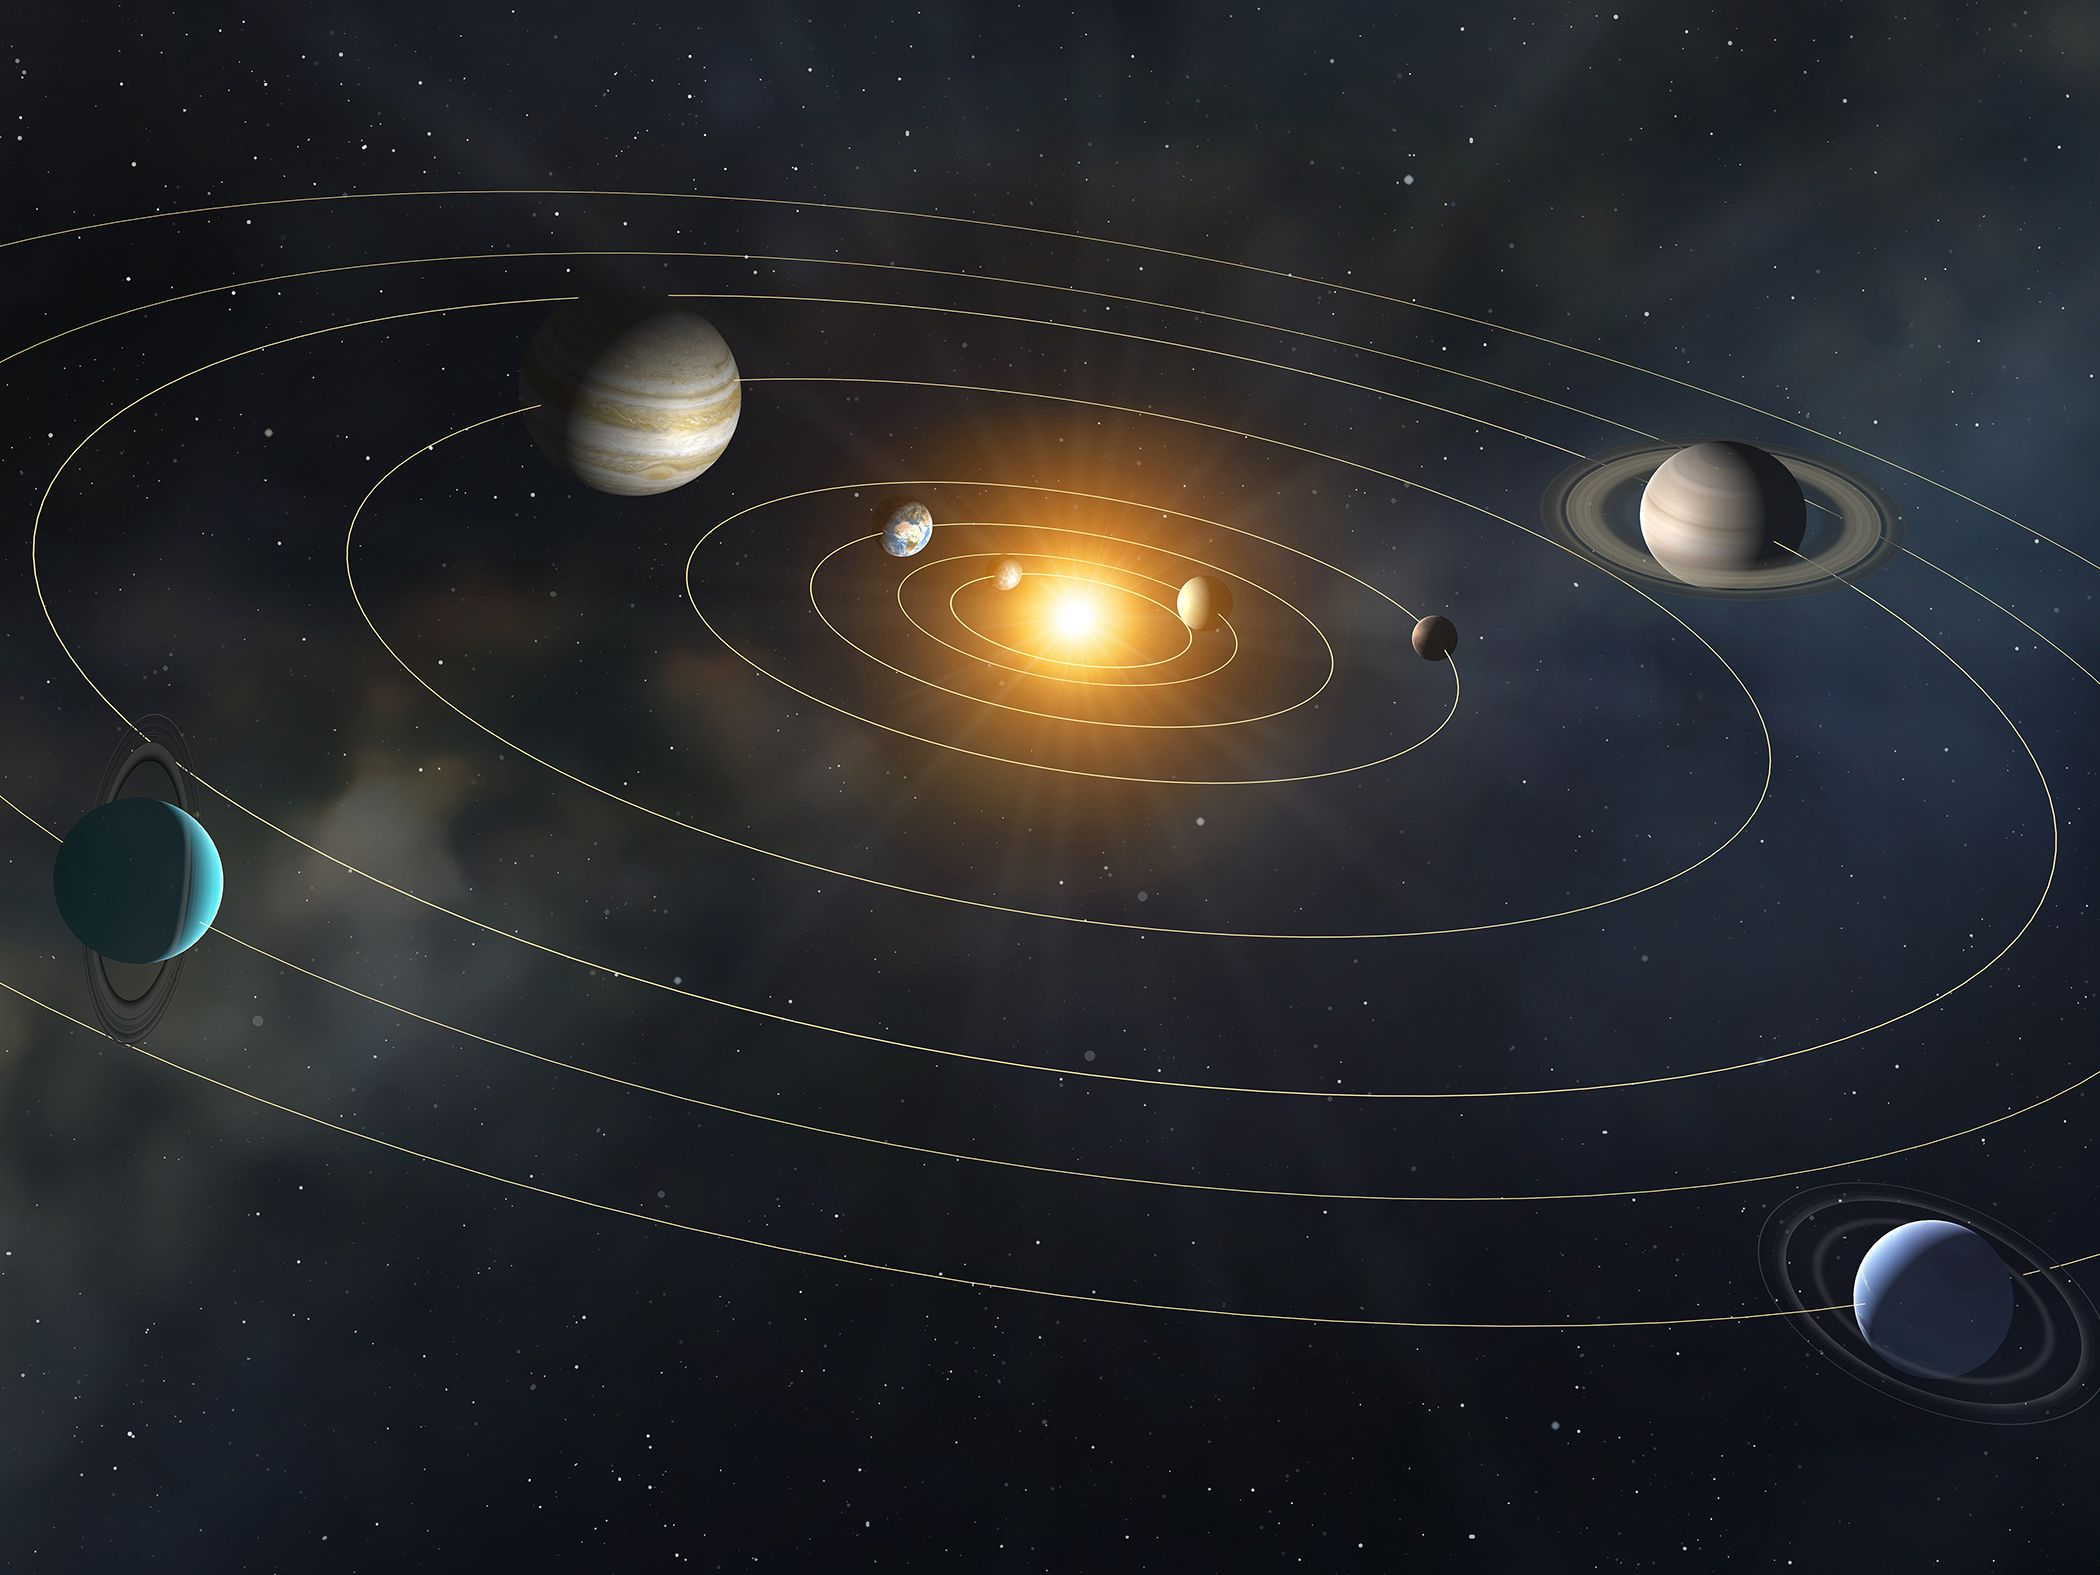
\includegraphics[width=0.8\textwidth,keepaspectratio]{Slides/Figure/solarsystem.jpg}
        \caption{Các hành tinh quay quanh Mặt Trời}
        \end{figure}
    \end{column}
    \begin{column}{0.5\textwidth}
        \begin{figure}
        \centering
        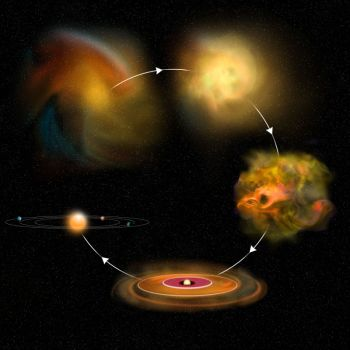
\includegraphics[width=0.6\textwidth,keepaspectratio]{Slides/Figure/planetformation.jpg}
        \caption{Sự hình thành sao và các hành tinh}
        \end{figure}
    \end{column}
    \end{columns}
\end{frame}

\begin{frame}
    \frametitle{Lực hấp dẫn}
    Ở một nơi trên bề mặt trái đất, trọng lực đối với một vật gần như không đổi, có chiều hướng từ trên xuống dưới mặt đất.
    \begin{columns}
    \begin{column}{0.5\textwidth}
        \begin{figure}
        \centering
        
\includegraphics[width=0.4\textwidth,keepaspectratio]{Slides/Figure/applefalling.jpg}
        \caption{Quả táo của Newton rơi do trọng lực}
        \end{figure}
    \end{column}
    \begin{column}{0.5\textwidth}
        Lực này có giá trị bằng:
        \begin{equation}
            F=mg
        \end{equation}
        trong đó \(F\) là lực hấp dẫn, \(m\) là khối lượng của vật, và \(g\) là gia tốc trọng trường (khoảng 9.81 m/s² trên bề mặt Trái Đất).
    \end{column}
    \end{columns}
\end{frame}

\begin{frame}
\frametitle{Lực điện từ}
\begin{tcolorbox}[colback=blue!10, colframe=blue!50!black, title=Định nghĩa]
Lực điện từ là lực tương tác giữa các hạt mang điện. Lực này bao gồm lực tĩnh điện, chịu trách nhiệm cho sự hút/đẩy của các điện tích trái dấu/cùng dấu; và lực từ do các điện tích chuyển động tạo ra.
\end{tcolorbox}
\begin{figure}
\centering
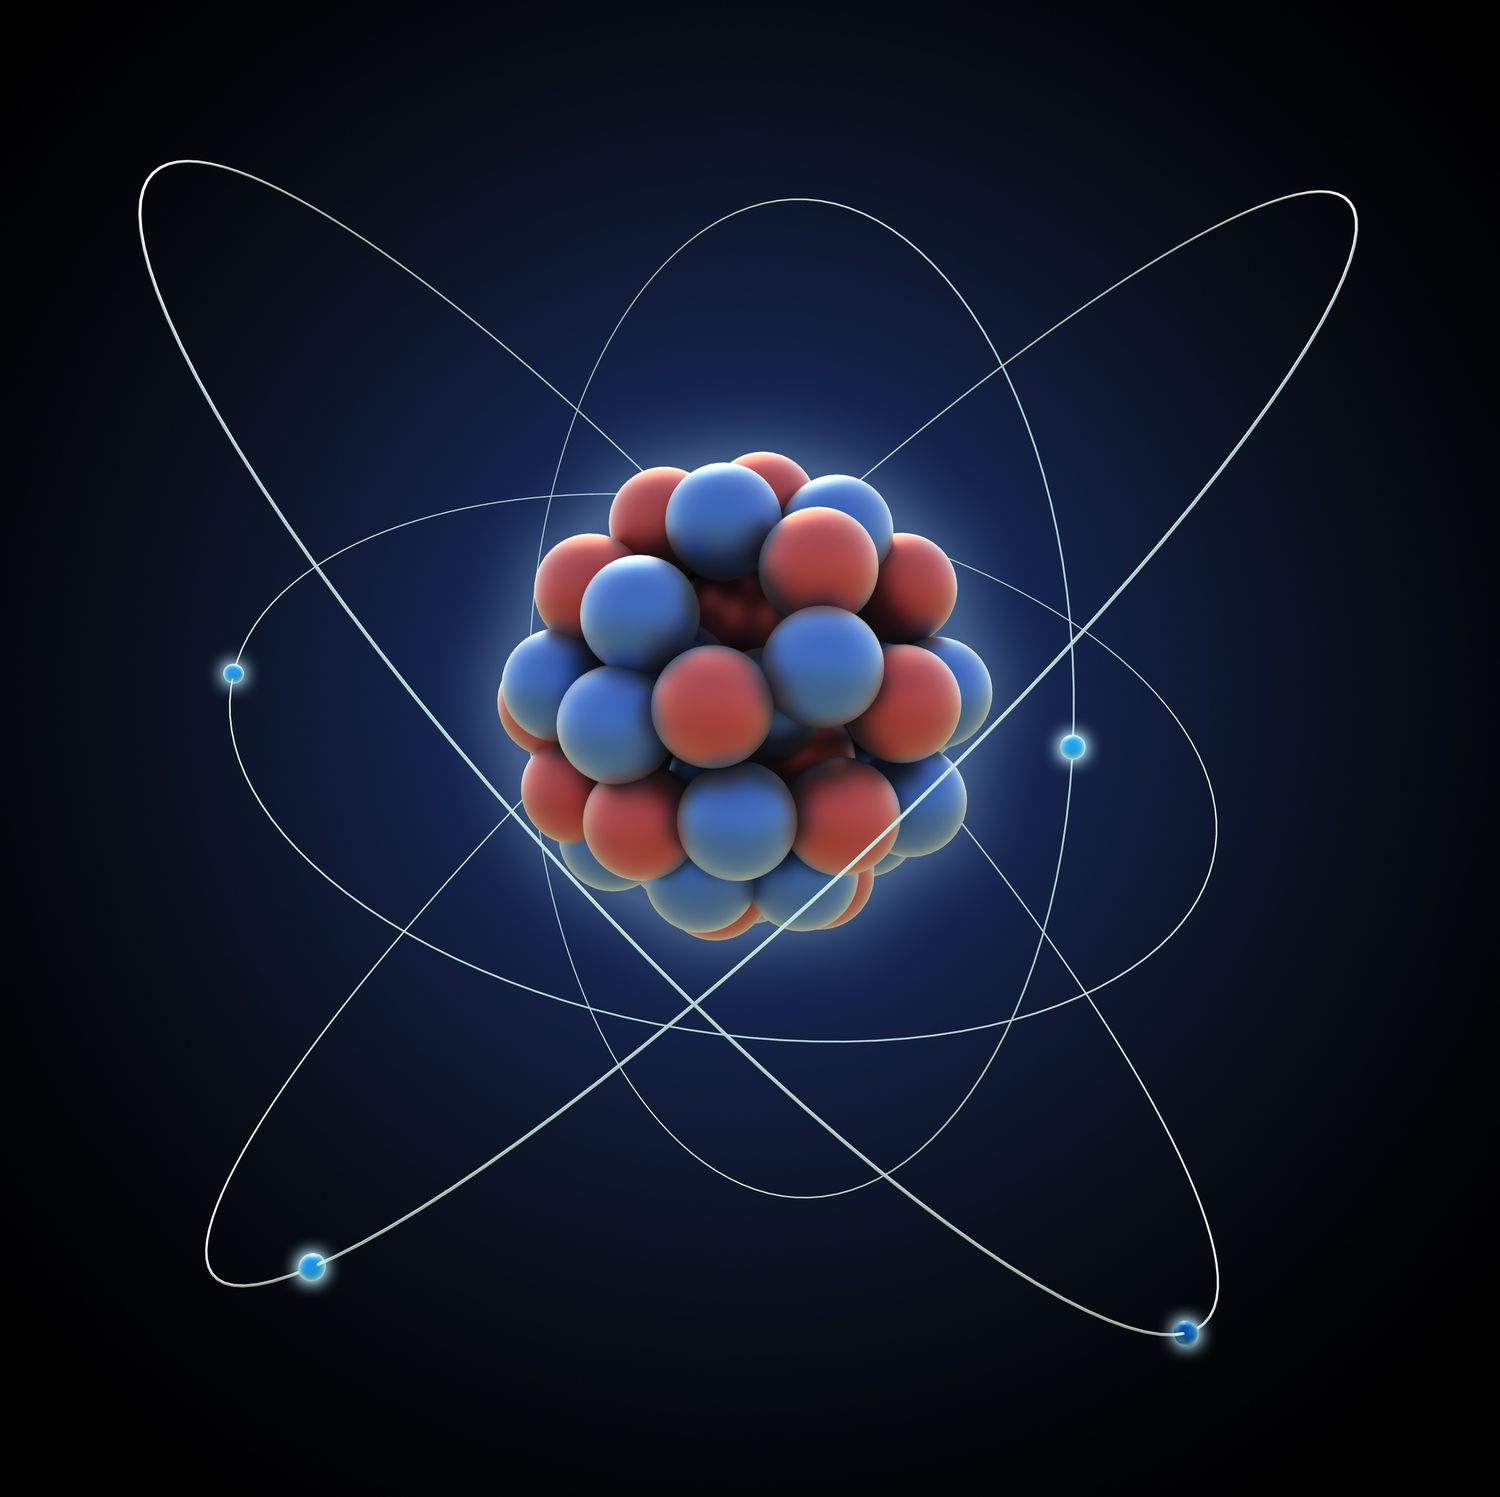
\includegraphics[width=0.15\textwidth]{Slides/Figure/atom.jpg}
\caption{Liên kết giữa các nguyên tử, phân tử}
\end{figure}
\end{frame}

\begin{frame}
\frametitle{Lực điện từ}
\begin{columns}
\begin{column}{0.5\textwidth}
    \begin{figure}
    \centering
    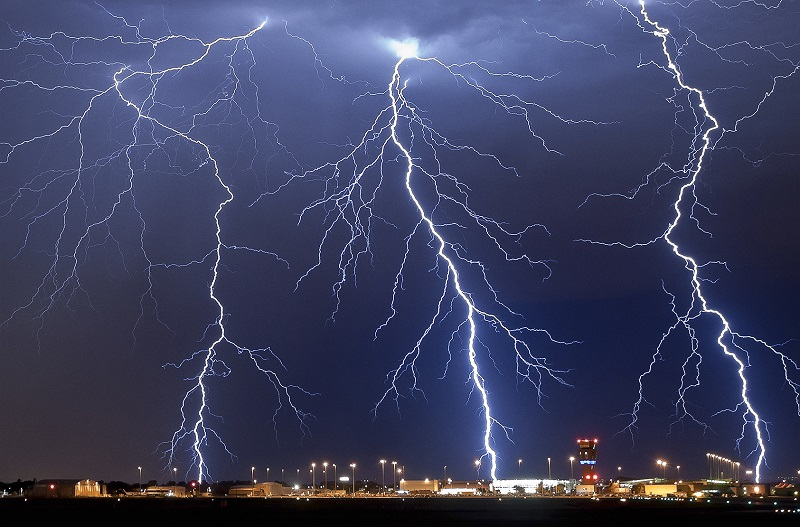
\includegraphics[width=0.775\textwidth]{Slides/Figure/thunder.jpg}
    \caption{Sấm sét}
    \end{figure}
\end{column}
\begin{column}{0.5\textwidth}
    \begin{figure}
    \centering
    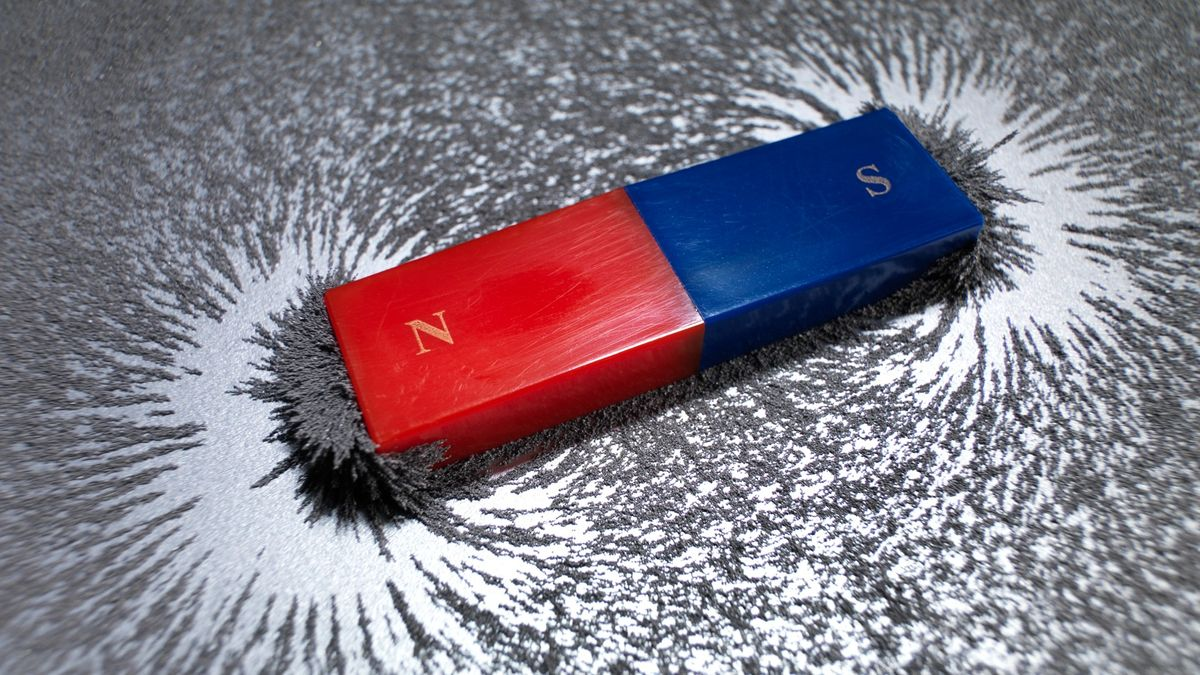
\includegraphics[width=0.9\textwidth]{Slides/Figure/magnet.jpg}
    \caption{Nam châm hút vụn sắt}
    \end{figure}
\end{column}
\end{columns}
\end{frame}

\subsection{Các lực vĩ mô}
\begin{frame}
    \frametitle{Lực đàn hồi}
    \textbf{Lực đàn hồi} xuất hiện khi một vật bị biến dạng và có xu hướng trở về hình dạng ban đầu. Đối với biến dạng không quá lớn, lực này tuân theo định luật Hooke:
    \begin{equation}
        F = -k \Delta x
    \end{equation}
    trong đó \(F\) là lực đàn hồi, \(k\) là hằng số đàn hồi, và \(\Delta x\) là độ biến dạng.
    \begin{figure}
        \centering
        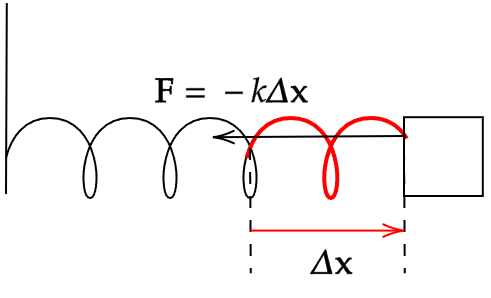
\includegraphics[width=0.3\textwidth]{Slides/Figure/springmass.png}
        \caption{Lực đàn hồi của lò xo}
    \end{figure}
\end{frame}

\begin{frame}
    \frametitle{Lực căng}
    Đối với các vật có hệ số đàn hồi rất lớn, tuy biến dạng nhỏ có thể không quan sát được nhưng vẫn có lực đàn hồi. Lực này gọi là \textbf{lực căng}, thường kí hiệu là \(T\).
    \begin{columns}
    \begin{column}{0.5\textwidth}
        \begin{figure}
        \centering
        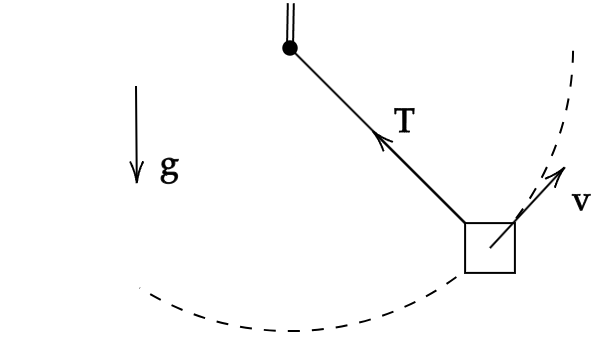
\includegraphics[width=0.6\textwidth]{Slides/Figure/rope.png}
        \end{figure}
        \begin{itemize}
            \item Lực căng dây \(T\) chống lại chuyển động theo phương song song với dây.
    \end{itemize}
    \end{column}
    \begin{column}{0.5\textwidth}
        \begin{figure}
        \centering
        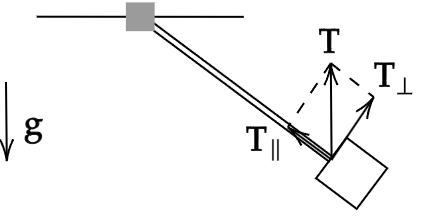
\includegraphics[width=0.5\textwidth]{Slides/Figure/rod.png}
        \end{figure}
        \begin{itemize}
            \item Lực căng thanh \(T_{\parallel}\) chống lại chuyển động theo phương song song với thanh.
            \item Lực căng thanh \(T_{\perp}\) chống lại sự bẻ cong của thanh.
        \end{itemize}
    \end{column}
    \end{columns}
\end{frame}

\begin{frame}
    \frametitle{Phản lực pháp tuyến}
Các mặt phẳng có thể sinh ra lực theo phương pháp tuyến với nó để chống lại sự chuyển động theo phương vuông góc với mặt phẳng này. Lực này được gọi là \textbf{phản lực pháp tuyến}.
\begin{figure}
\centering
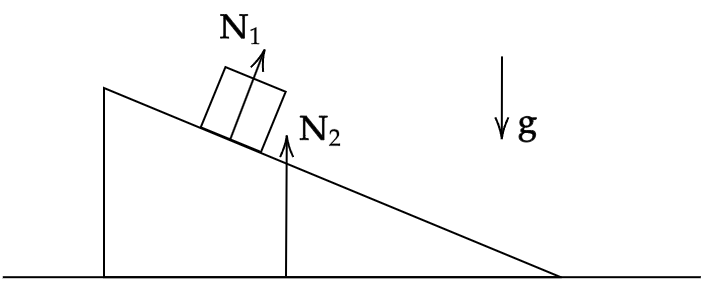
\includegraphics[width=0.5\textwidth]{Slides/Figure/wedge.png}
\caption{Phản lực pháp tuyến của các mặt phẳng}
\end{figure}
\end{frame}

\begin{frame}
    \frametitle{Lực ma sát}
    \begin{columns}
    \begin{column}{0.5\textwidth}
    Các khuyết tật trên bề mặt có thể sinh ra phản lực theo phương song song với các bề mặt này khi chúng tiếp xúc với nhau. Lực này được gọi là \textbf{lực ma sát}.
    \begin{figure}
        \centering
        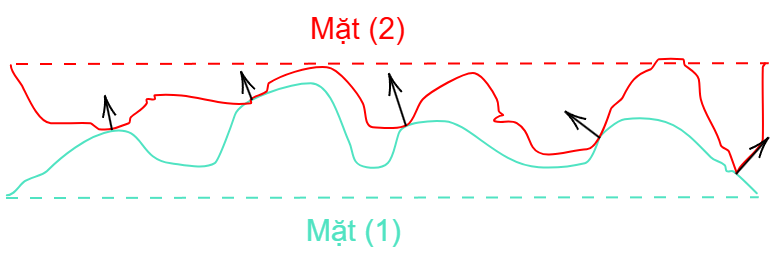
\includegraphics[width=0.9\textwidth]{Slides/Figure/friction.png}
        \caption{Lực ma sát giữa các bề mặt tiếp xúc}
    \end{figure}
    \end{column}
    \begin{column}{0.5\textwidth}
    Lực mà sát tỉ lệ thuận với phản lực pháp tuyến giữa hai bề mặt:
    \begin{equation}
        F_{ms} = \mu N
    \end{equation}
    trong đó \(F_{ms}\) là lực ma sát, \(\mu\) là hệ số ma sát, và \(N\) là phản lực pháp tuyến.
    \begin{figure}
        \centering
        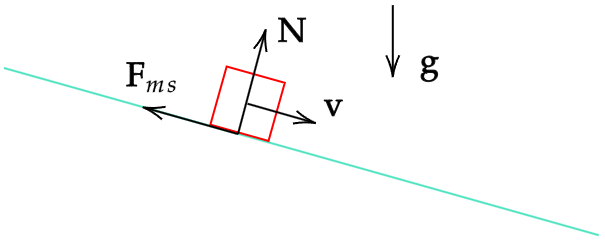
\includegraphics[width=0.7\textwidth]{Slides/Figure/slope.png}
        \caption{Lực ma sát giữa vật và mặt phẳng nghiêng}
    \end{figure}
    \end{column}
    \end{columns}
\end{frame}